62. $\cfrac{x}{x+1}-\cfrac{2x}{x^2-x+1}\geqslant\cfrac{x-2x^2}{x^3+1}\Leftrightarrow \cfrac{x^3-x^2+x-2x^2-2x-x+2x^2}{(x+1)(x^2-x+1)}\geqslant0
\Leftrightarrow \cfrac{x(x+1)(x-2)}{(x+1)(x^2-x+1)}\geqslant0.$ Применив метод интервалов, найдём ответ: $x\in (-\infty;-1)\cup(-1;0]\cup[2;+\infty).$
\begin{figure}[ht!]
\center{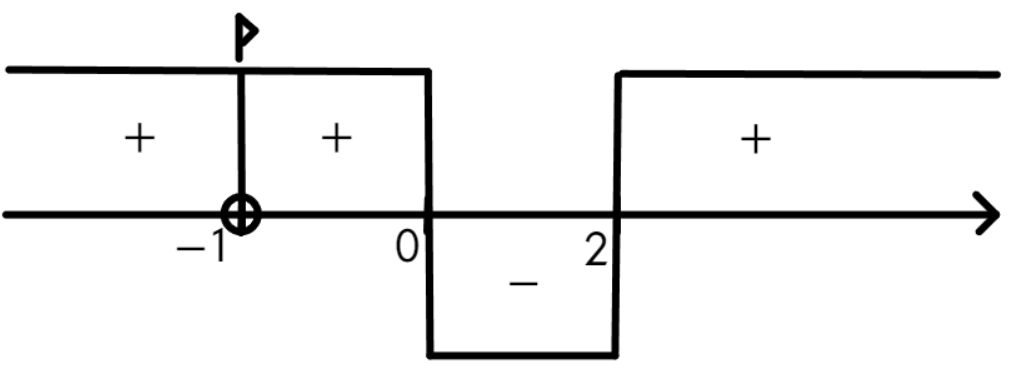
\includegraphics[scale=0.35]{ner9-62.png}}
\end{figure}\\
